\documentclass[12pt,letterpaper]{report}
\usepackage{pgf, tikz}
\usetikzlibrary{arrows, mindmap,graphs,automata,shapes.geometric,intersections}
\usetikzlibrary{positioning}
\begin{document}
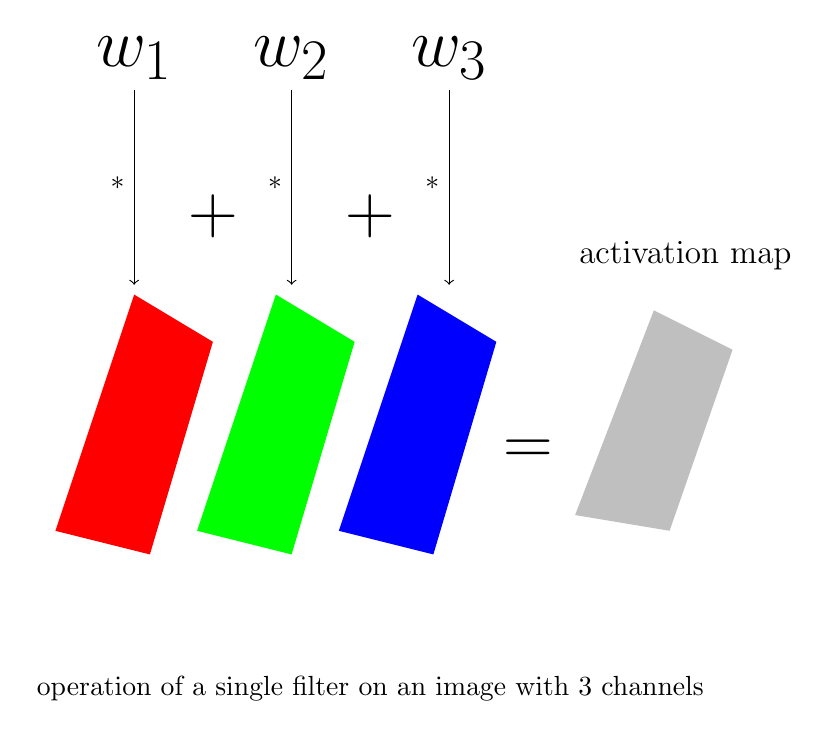
\begin{tikzpicture}
    \node (w1) at (1,6) {\Huge $w_1$};
    \node (w2) at (3,6) {\Huge $w_2$};
    \node (w3) at (5,6) {\Huge $w_3$};
    \node (anc1) at (1,3) {};
    \node (anc2) at (3,3) {};
    \node (anc3) at (5,3) {};
    \node (add1) at (2,4) {\Huge +};
    \node (add2) at (4,4) {\Huge +};

    \path[->] (w1) edge node[left]{*} (anc1);
    \path[->] (w2) edge node[left]{*} (anc2);
    \path[->] (w3) edge node[left]{*} (anc3);

    \coordinate (a) at (0,0);
     \coordinate (b) at (1,3);
     \coordinate (c) at (2,2.4);
     \coordinate (d) at (1.2,-0.3);
    \filldraw[draw=none,fill=red] (a) -- (b) -- (c) -- (d) -- (a);


    \coordinate (a1) at (1.8,0);
    \coordinate (b1) at (2.8,3);
    \coordinate (c1) at (3.8,2.4);
    \coordinate (d1) at (3,-0.3);
   \filldraw[draw=none,fill=green] (a1) -- (b1) -- (c1) -- (d1) -- (a1);
    %\filldraw[fill=red] (a) circle (2);

    \coordinate (a2) at (3.6,0);
    \coordinate (b2) at (4.6,3);
    \coordinate (c2) at (5.6,2.4);
    \coordinate (d2) at (4.8,-0.3);
   \filldraw[draw=none,fill=blue] (a2) -- (b2) -- (c2) -- (d2) -- (a2);
    %\filldraw[fill=red] (a) circle (2);

\node (eq) at (6,1) {\Huge =};
    \coordinate (a3) at (6.6,0.2);
    \coordinate (b3) at (7.6,2.8);
    \coordinate (c3) at (8.6,2.3);
    \coordinate (d3) at (7.8,0);
   \filldraw[draw=none,fill=lightgray] (a3) -- (b3) -- (c3) -- (d3) -- (a3);
   \node (label) at (4,-2) {operation of a single filter on an image with 3 channels};
   \node (amap) at (8,3.5) {\large activation map};
\end{tikzpicture}
\end{document}